\chapter{Methods}
\label{chp:methods}


%% Vi kan sikkert skrive litt om dette i metode

% \subsection{Version Control}
% \label{subsec:version-control}

% The use of \gls{git} as a version control system enables collaborative development by allowing multiple developers to work on the same codebase simultaneously. \gls{git} facilitates the maintenance of the code and provides a comprehensive history of all modifications made to the project. These changes are tracked within project containers known as \glspl{repository}, ensuring transparency and accountability throughout the development process. \cite{alphaefficiency:git}

% \subsubsection*{Branches}

% Git utilizes branches, which are independent lines of development within a repository. Branches allow developers to work on new features, fixes, or experiments without affecting the main codebase. Once changes in a branch are tested and finalized, they can be merged back into the main branch, ensuring a streamlined and controlled integration process. Branching supports parallel development and helps prevent conflicts by isolating work until it's ready for review and integration. \cite{git:branches}

\begin{center}
    \textit{Here, the development process and methodologies are described in detail. This includes the design and implementation of the desktop application, the selection of tools and frameworks, and the approach to solving the problem.}
\end{center}



\section{Machine Learning Models}
\label{sec:ml-models}

After conducting research into existing chess digitization methods, a publicly available solution developed by Peter Batchelor, Tom Richardson, and other contributors was discovered. This solution served as the foundation for the approach. It utilized two \glspl{cnn}: one for detecting chess pieces and another for locating the squares of the chessboard \cite{lichess:chesscam}. \\

Although the documentation for the models was limited, the necessary logic and structure of the models were already present in the repository itself. When additional clarifications were needed, they were obtained through direct communication with the original developers, ensuring that the intended use and functionality of the models were correctly understood. \\

The ChessCam repository provided multiple model formats, including PyTorch and \gls{onnx}. Before the models could be used, it was necessary to understand their expected inputs and outputs. Netron was employed to inspect the \gls{onnx} files and determine these details. \\


\subsection{Piece Detection Model}
The piece detection model was responsible for identifying and classifying chess pieces on the board. It expected \textbf{input} in the format \textbf{[1, 3, 288, 480]}. \textbf{1} represented the batch size, i.e. the number of images processed at once. \textbf{3} corresponded to the number of color channels (RGB), indicating that the image had to be in color. \textbf{288} and \textbf{480} denoted the height and width of the image in pixels, respectively. \\

The piece model output data in the format \textbf{[1, 16, 2835]}. \textbf{1} represented the batch size. \textbf{2835} represented the number of anchor boxes used in the detection and \textbf{16} consisted of two parts: \\

The first 4 values were offset values that adjusted the position and size of each anchor box to better align with a detected piece. These offsets were relative to the predefined anchor boxes, as illustrated in Table \ref{tab:piece-offset-table}.

\begin{table}[h]
    \centering
    \caption[Example offset values for anchor boxes - chess pieces]{Offset coordinates for each anchor box with regard to identifying chess pieces.}  % Caption moved to top
    \renewcommand{\arraystretch}{1.5} % Increase row height to allow text to be on top
    \begin{tabular}{lcccc}
        \toprule
        \textbf{Anchor box} & \textbf{xcenter} & \textbf{ycenter} & \textbf{width} & \textbf{height} \\
        \midrule
        Anchor box 1 & -3.23 & 0.57 & -0.12 & -0.34 \\
        Anchor box 2 & 0.51 & -0.63 & 4.15 & 1.27 \\
        Anchor box 3 & 7.71 & 0.29 & -0.11 & 2.45 \\
        ... & ... & ... & ... & ... \\
        Anchor box 2835 & -0.04 & 2.11 & 1.15 & 5.32 \\
        \bottomrule
    \end{tabular}
    \label{tab:piece-offset-table}
\end{table}


The remaining 12 values represented the probabilities for each possible piece type after the offset value had been applied. With 12 different piece types, the model output 12 probabilities for each anchor box. The classification labels are shown in Table \ref{tab:piece-label-table}. Table \ref{tab:piece-probability-table} presents the predicted probabilities for each label across all anchor boxes. \\
\begin{table}[ht]
\renewcommand{\arraystretch}{1.2}  % Increase row height slightly
\centering
\caption[Labels for chess piece types]{Classification labels for the 12 chess piece types predicted by the model.}
\begin{tabular}{|c|c|}
\hline
\multicolumn{2}{|c|}{\textbf{Model Labels}} \\  
\hline
\textbf{Black Pawn} & \textbf{White Pawn} \\
\textbf{Black Knight} & \textbf{White Knight} \\
\textbf{Black Bishop} & \textbf{White Bishop} \\
\textbf{Black Rook} & \textbf{White Rook} \\
\textbf{Black Queen} & \textbf{White Queen} \\
\textbf{Black King} & \textbf{White King} \\
\hline
\end{tabular}
\label{tab:piece-label-table}
\end{table}


\\


\begin{table}[h]
    \centering
    \caption[Predicted chess piece type after applying offsets]{Predicted class probabilities for each anchor box after applying the offsets.}  % Caption moved to top
    \renewcommand{\arraystretch}{1.5}
    \begin{tabular}{lcccc}
        \toprule
        \textbf{Anchor box} & \textbf{Black Pawn} & \textbf{White Pawn} & \textbf{Black Knight} & \textbf{...} \\
        \midrule
        Anchor box 1 & \raggedright 0.03 & \raggedright 0.71 & \raggedright 0.01 & ... \\
        Anchor box 2 & \raggedright 0.82 & \raggedright 0.02 & \raggedright 0.01 & ... \\
        Anchor box 3 & \raggedright 0.02 & \raggedright 0.01 & \raggedright 0.78 & ... \\
        ... & ... & ... & ... & ... \\
        Anchor box 2835 & \raggedright 0.01 & \raggedright 0.03 & \raggedright 0.05 & ... \\
        \bottomrule
    \end{tabular}
    \label{tab:piece-probability-table}
\end{table}

There were 2835 predefined anchor boxes spread across the image, each serving as a candidate location for detecting a chess piece. During training, the model learned to adjust these anchor boxes to better match the actual pieces on the board. It achieved this by predicting 4 offset values that modified the location and size of each anchor box. At runtime, for each anchor box, the model used these learned offsets and output 12 class probabilities, indicating the likelihood of each chess piece type being present at that location.

\newpage

\subsection{Corner Detection Model}
The corner detection model identified the points where the edges of the inner squares on the chessboard met, commonly referred to as intersection points. Up to 49 intersection points could be detected in a single image. These points are illustrated in Figure \ref{fig:xcorners-chessboard}.

\begin{figure}[h!]
    \centering
    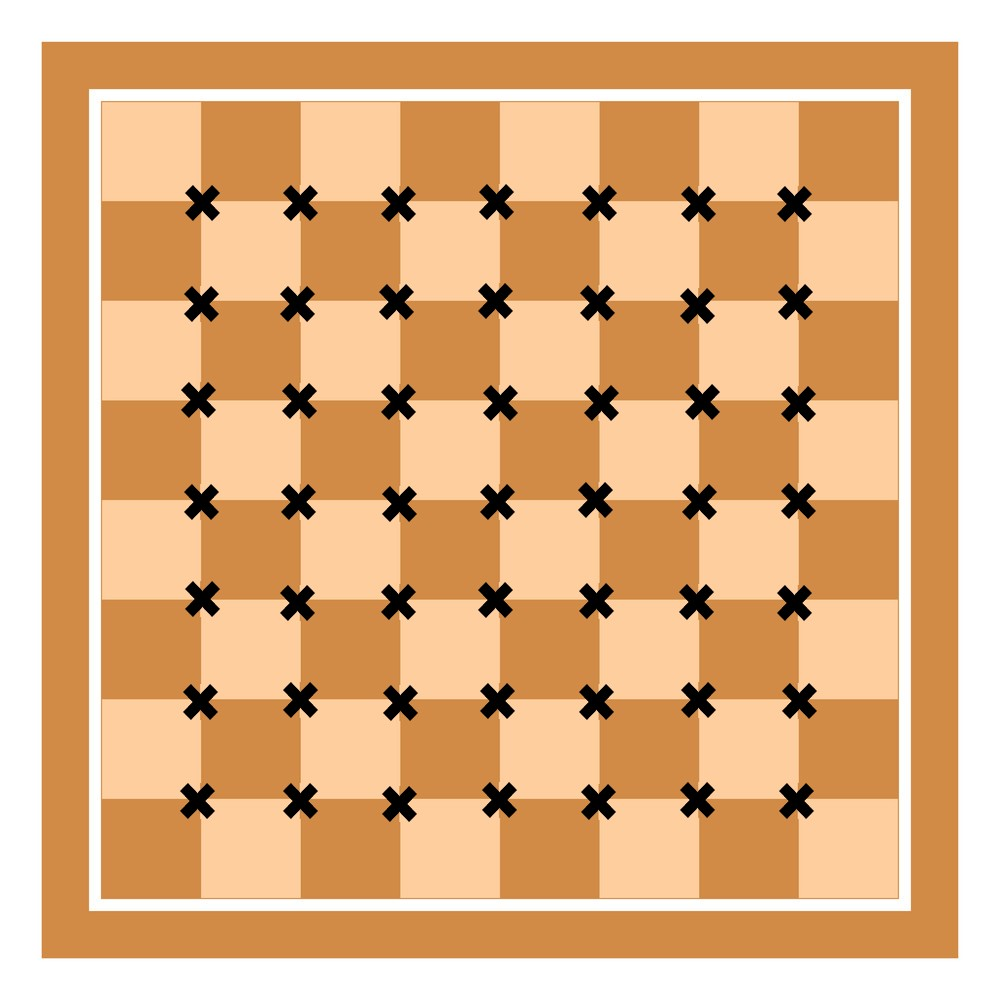
\includegraphics[width=0.75\linewidth]{figures/methods/ml-models/xcorners_chessboard.jpg}
    \caption[Detected intersection points on chessboard]{Visualization of intersection points where the edges of the inner squares on the chessboard meet. The model identified and predicted these points. Up to 49 intersection points could be detected in a single image. \cite{vectorstock:chessboard-svg}}
    \label{fig:xcorners-chessboard}
\end{figure}

The input for the corner model was the same as the piece model: \textbf{[1, 3, 288, 480]}. The corner model output predictions in the format \textbf{[1, 5, 2835]}. \textbf{1} represented the batch size. \textbf{2835} represented the number of anchor boxes used in the detection. \textbf{5} consisted of two parts: \\

The first 4 values were offset values that adjusted the position and size of each anchor box, aligning it more accurately with a potential intersection point. These offsets were relative to the original anchor box coordinates, as shown in Table \ref{tab:corner-offset-table}.

% \newpage

\begin{table}[h]
    \centering
    \caption[Offset values for anchor box - intersection points]{Example offset coordinates for each anchor box with regard to identifying intersection points.}  % Caption moved to top
    \renewcommand{\arraystretch}{1.5} % Increase row height to allow text to be on top
    \begin{tabular}{lcccc}
        \toprule
        \textbf{Anchor box} & \textbf{xcenter} & \textbf{ycenter} & \textbf{width} & \textbf{height} \\
        \midrule
        Anchor box 1 & -1.43 & 3.27 & -0.52 & -2.21 \\
        Anchor box 2 & 2.51 & -7.61 & 0.15 & 4.17 \\
        Anchor box 3 & -3.71 & 1.49 & -4.21 & 2.45 \\
        ... & ... & ... & ... & ... \\
        Anchor box 2835 & -2.04 & 3.29 & -0.35 & 1.24 \\
        \bottomrule
    \end{tabular}
    \label{tab:corner-offset-table}
\end{table}

The final value was the probability that the adjusted anchor box corresponded to an intersection point on the chessboard, as illustrated in Table~\ref{tab:corner-probability-table}. \\

\begin{table}[h]
    \centering
    \caption[Predicted intersection points after applying offsets]{Predicted intersection probabilities for each anchor box after applying the offsets.}
    \renewcommand{\arraystretch}{1.5}
    \begin{tabular}{lc}
        \toprule
        \textbf{Anchor Box} & \textbf{Intersection Probability} \\
        \midrule
        Anchor Box 1 & 0.06 \\
        Anchor Box 2 & 0.91 \\
        Anchor Box 3 & 0.03 \\
        ... & ... \\
        Anchor Box 2835 & 0.87 \\
        \bottomrule
    \end{tabular}
    \label{tab:corner-probability-table}
\end{table}


% \newpage


\subsection{Combining The Models}

To track chess piece movements, the first step was to identify the individual squares of the chessboard. Once the squares were identified, each detected piece needed to be mapped to its corresponding square. This required determining the outer corners of the chessboard. With the corners identified, the board was divided into an 8x8 grid of equally sized squares. Since the distance between the corners was known and all squares in the grid are of uniform size, the centers of the squares could be precisely calculated. For each square, only the center point would be used for subsequent mapping, as shown in Figure~\ref{fig:chessboard-centers}.



\begin{figure}[h!]
    \centering
    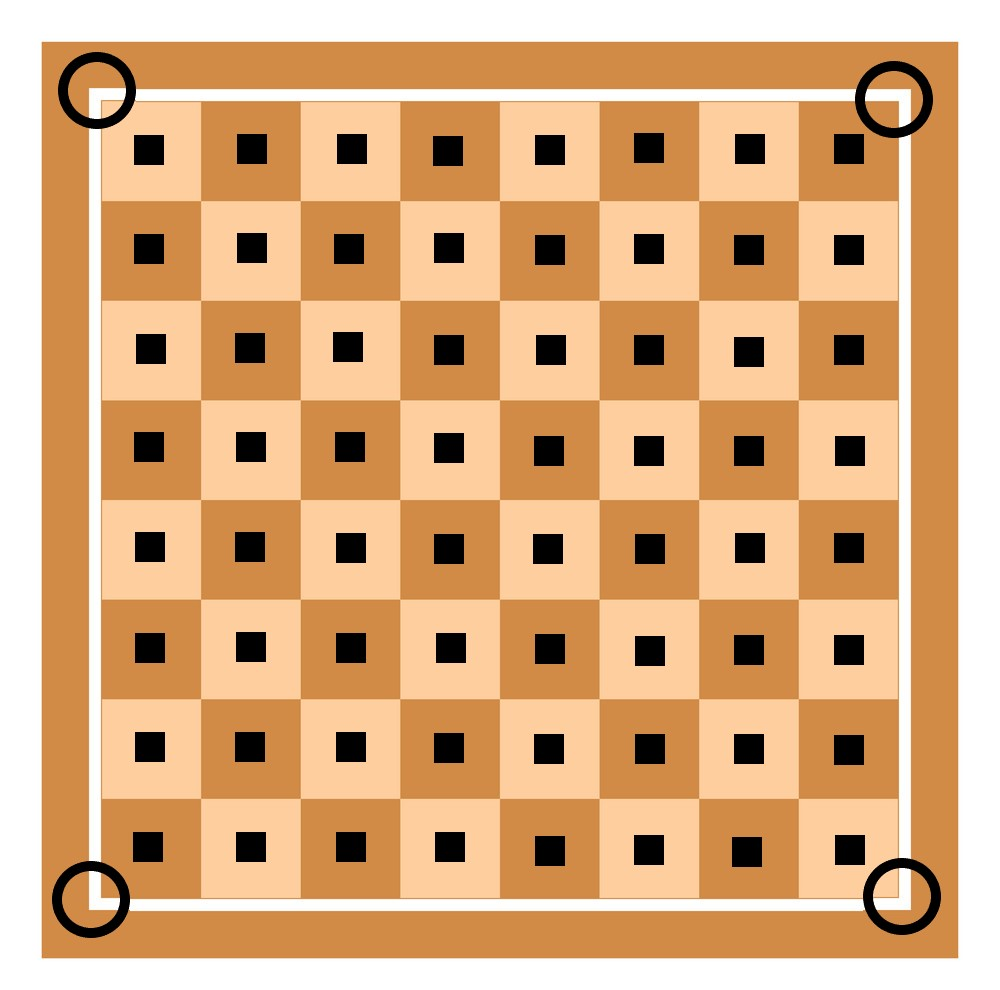
\includegraphics[width=0.75\linewidth]{figures/methods/ml-models/outer_corners_centers_chessboard.jpg}
    \caption[Chessboard corners and centers]{Visualization of the corners of the chessboard and the centers of each individual square, forming an 8x8 grid. \cite{vectorstock:chessboard-svg}}
    \label{fig:chessboard-centers}
\end{figure}


The bottom center of each piece’s bounding box was selected as its representative location, as highlighted in Figure~\ref{fig:bbox-black-pawn}. Each detected piece was then mapped to the nearest square center based on the minimum euclidean distance.  This approach made it possible to accurately assign each piece to a specific square on the chessboard.


% \newpage


\begin{figure}[h!]
    \centering
    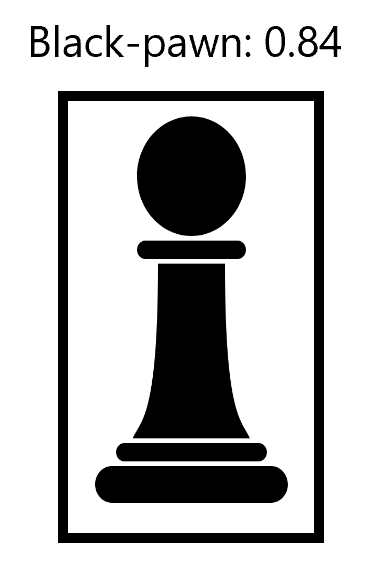
\includegraphics[width=0.25\linewidth]{figures/methods/ml-models/black-pawn.png}
    \caption[Detected chess piece and its bounding box]{Example of a detected chess piece with its classification confidence. The bottom center of the bounding box was used as the reference point for mapping the piece to its corresponding square. \cite{svgrepo:black-pawn-svg}}
    \label{fig:bbox-black-pawn}
\end{figure}


\subsubsection*{Board Detection}

Each frame captured by the camera was processed by the two models. Before inference, the frame needs to match the models’ expected input dimensions [1, 3, 288, 480]. This process includes scaling the frame, normalizing the pixel values to fall within the range [0, 1] and converting the image to the appropriate data type. \\

After inference, the models produce the prediction outputs: [1, 16, 2835] for pieces and [1, 5, 2835] for intersection points. These outputs represent 2835 potential locations for both chess pieces and intersection points. To identify the most reliable predictions, low-confidence entries are first filtered out. Furthermore, NMS was applied to further refine the results. This process ensures only the most accurate locations for the pieces and intersections were retained. \\

To identify the board corners of the chessboard, Delaunay triangulation was used. Delaunay triangulation was applied to the intersection points to generate a set of candidate triangles. By iterating over these triangles and examining their shared vertices, the algorithm identifies potential quadrilaterals (four-sided shapes) that represent the four corners of the chessboard. Once a list of candidate quadrilaterals was generated, each was scored based on how well it fit the original intersection points. The quadrilateral with the highest score was then selected as the most likely representation of the board corners.
\\

With the corners identified, the next step was to correct the distortion caused by the camera angle. When viewed at an angle, the board appears skewed due to varying distances between the camera and different parts of the board. This distortion can be corrected by using a perspective transformation. Specifically, the inverse of the transformation matrix responsible for the distortion is computed. By applying this inverse to the distorted image, the transformation that warped the image is reversed, effectively 'flattening' the distorted chessboard back to its ideal, top-down view. Once the inverse matrix is applied, the resulting coordinates provide the corrected positions of the corners in the distorted image. \\

With the distortion corrected, the board is treated as an 8×8 grid of uniformly sized squares, each occupying a unit-length cell. The center of each square lies midway between its edges, resulting in center coordinates that range from 0.5 to 7.5 in both the x and y axes. The center of the first square is at (0.5, 0.5), the second at (1.5, 0.5), and so on up to (7.5, 7.5). \\

To finalize the board orientation, the average center of all black and white pieces was computed. The board was then rotated in four 90-degree increments. For each rotation, the midpoints of the expected white and black sides were calculated as the average coordinates between pairs of corners. Specifically, the midpoint for the white side was calculated between ‘a1’ and ‘h1’, and for the black side between ‘a8’ and ‘h8’. The rotation minimizing the distance between piece centers and these midpoints was selected as the correct alignment. Based on this orientation, the labels ‘a1’, ‘h1’, ‘a8’, and ‘h8’ were assigned to the corners of the chessboard. A visualization of this process is shown in Figure~\ref{fig:board_label_assignment}.
 
% \newpage

\begin{figure}[h!]
\centering
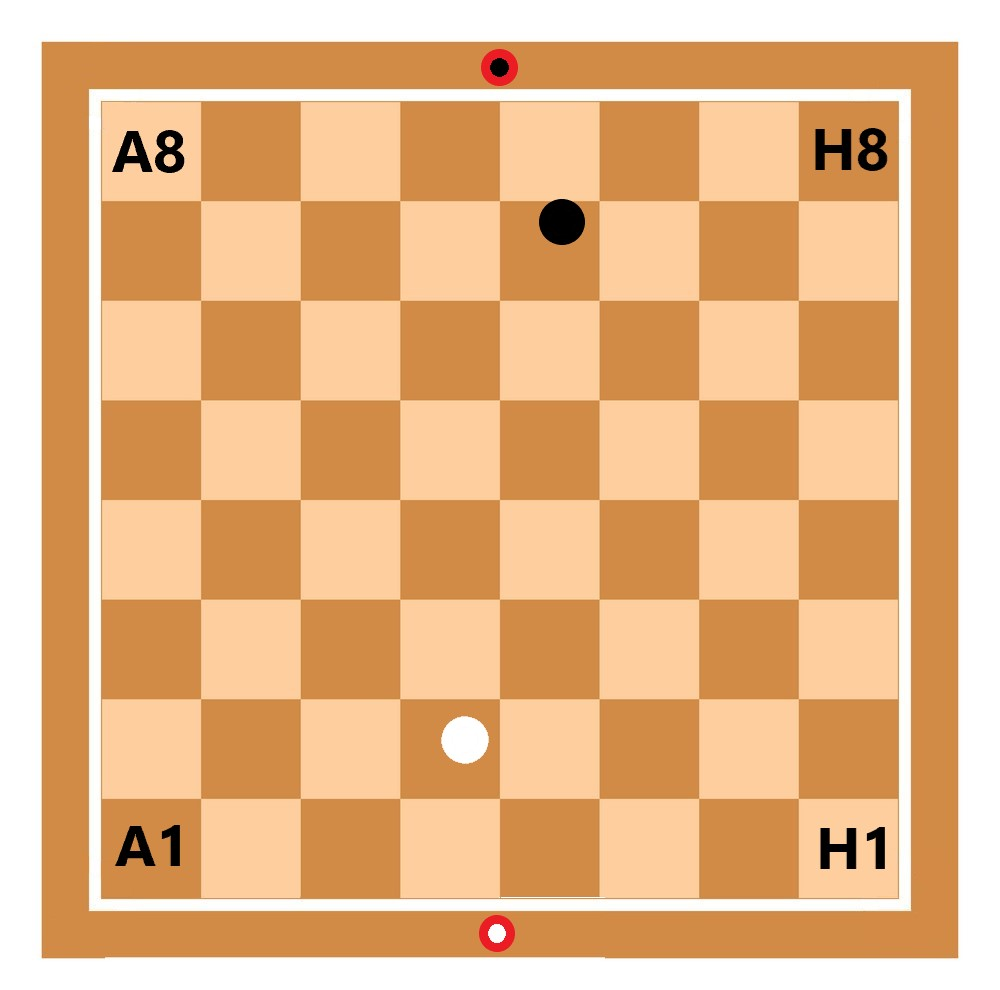
\includegraphics[width=0.70\linewidth]{figures/methods/ml-models/label_assignment_board.jpg}
\caption[Assigning labels to chessboard]{The white and black circles represent the average centers of the white and black pieces. The red circles indicate the midpoints between the corners on the white and black sides. The board is rotated, and the labels are assigned based on the rotation that minimizes the distance between the centers and the midpoints.}
\label{fig:board_label_assignment}
\end{figure}


\subsubsection*{Move detection}

After the chessboard and pieces have been detected, the application continuously processes each incoming video frame to detect whether a move has occurred. For every frame, the internal representation of the board state is updated based on the observed positions of the chess pieces. \\

To ensure stability, the system updates its internal state using a decay-based mechanism that blends previous and current detections. This approach smooths out transient errors due to occlusions or momentary inconsistencies in the video feed. State updates are throttled to occur at fixed intervals, which reduces the frequency of updates and helps maintain performance while avoiding unnecessary processing during minor fluctuations in detection. \\

Once the updated configuration is established, the system compares it against the legal move set of the current game state. If a high-confidence match is found, the move is registered and applied. Upon confirming a move it is committed to the internal chess engine and sent to the websocket for it to send to the frontend. The game state is updated accordingly for continued analysis and visualization.\\

\begin{figure}[h!]
    \centering
    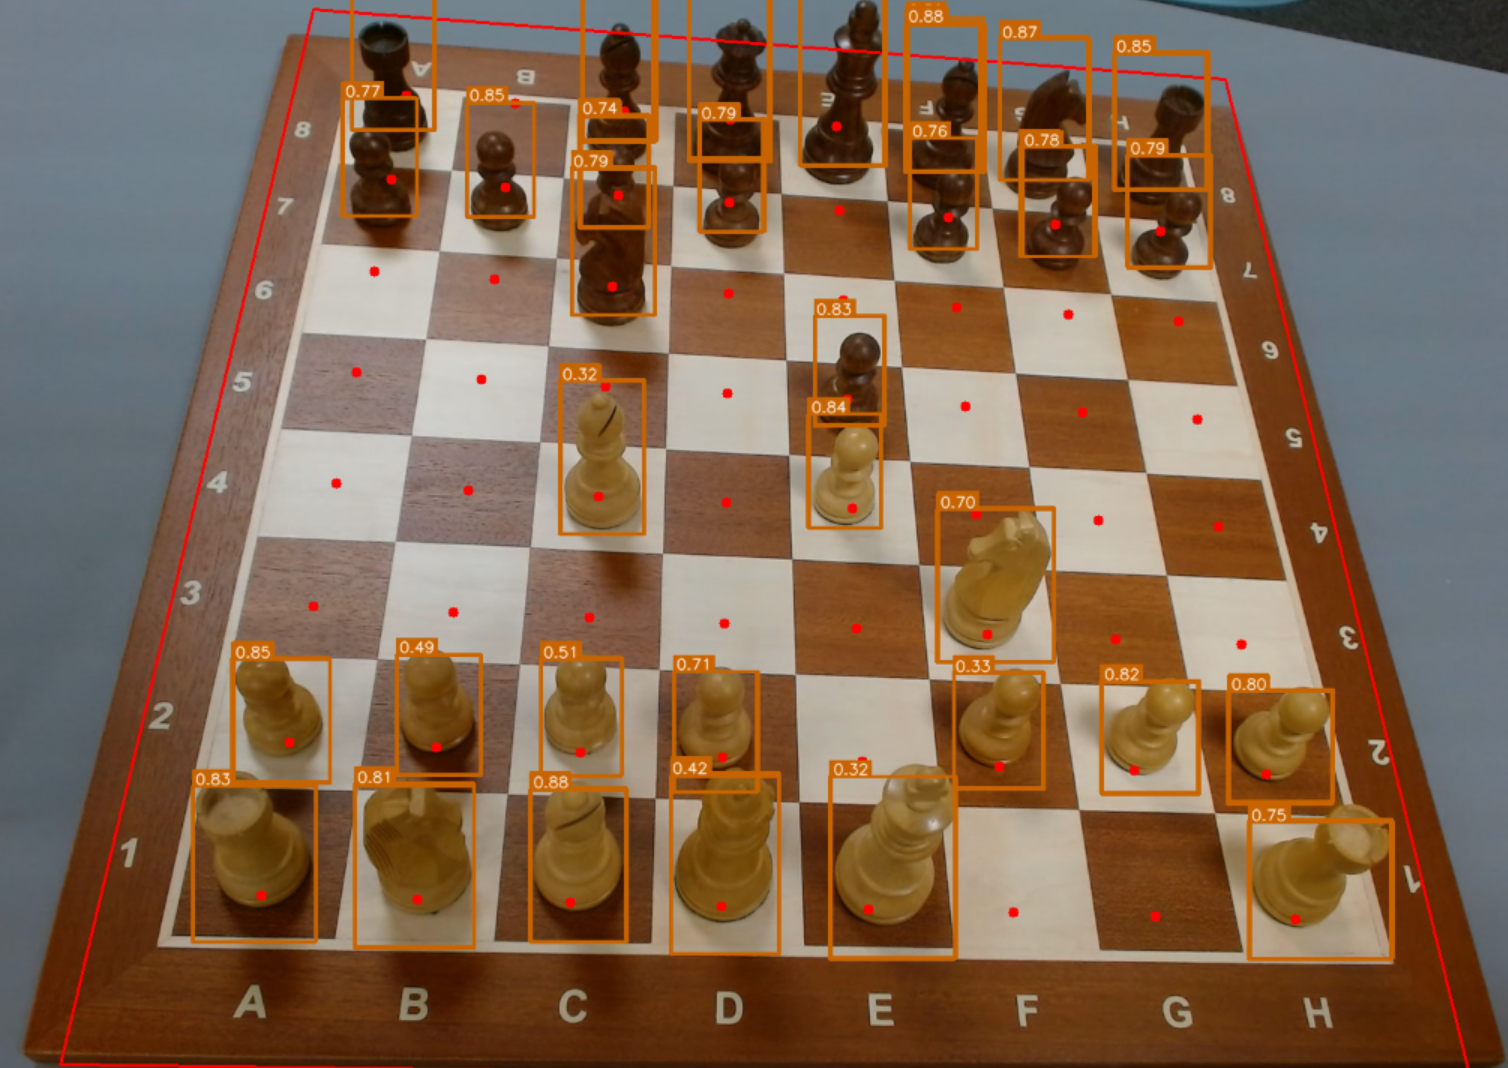
\includegraphics[width=0.75\linewidth]{figures/methods/ml-models/piece-model.png}
    \caption[Visualization of piece model and corner model]{Visualization of the detected pieces and centers of the squares.}
    \label{fig:websocket-vs-http}
\end{figure}

\section{Design}

\subsection{Wireframes}
\label{subsec:wireframe}

\subsubsection*{Control Panel}

The Control Panel is a desktop interface for tournament organizers to manage the digitization of multiple physical chess boards. It follows a simple three-step workflow:

\begin{enumerate}
\item \textbf{Select Number of Cameras:} Specify the number of boards to monitor, which determines how many camera feeds are initialized (Figure \ref{fig:control-panel-1}).
\item \textbf{Start Cameras and Digitization:} Launches the camera feeds, board state recognition, and move validation (Figure \ref{fig:control-panel-2}).
\item \textbf{Restart Boards for New Round:} Resets all boards at the end of a round, preparing the system for the next games (Figure \ref{fig:control-panel-3}).
\end{enumerate}

The interface is minimal and task-focused, enabling efficient system setup and management with little technical effort. \\

\newpage

\begin{figure}[h!]
    \centering
    \begin{subfigure}[h!]{0.40\linewidth}
        \centering
        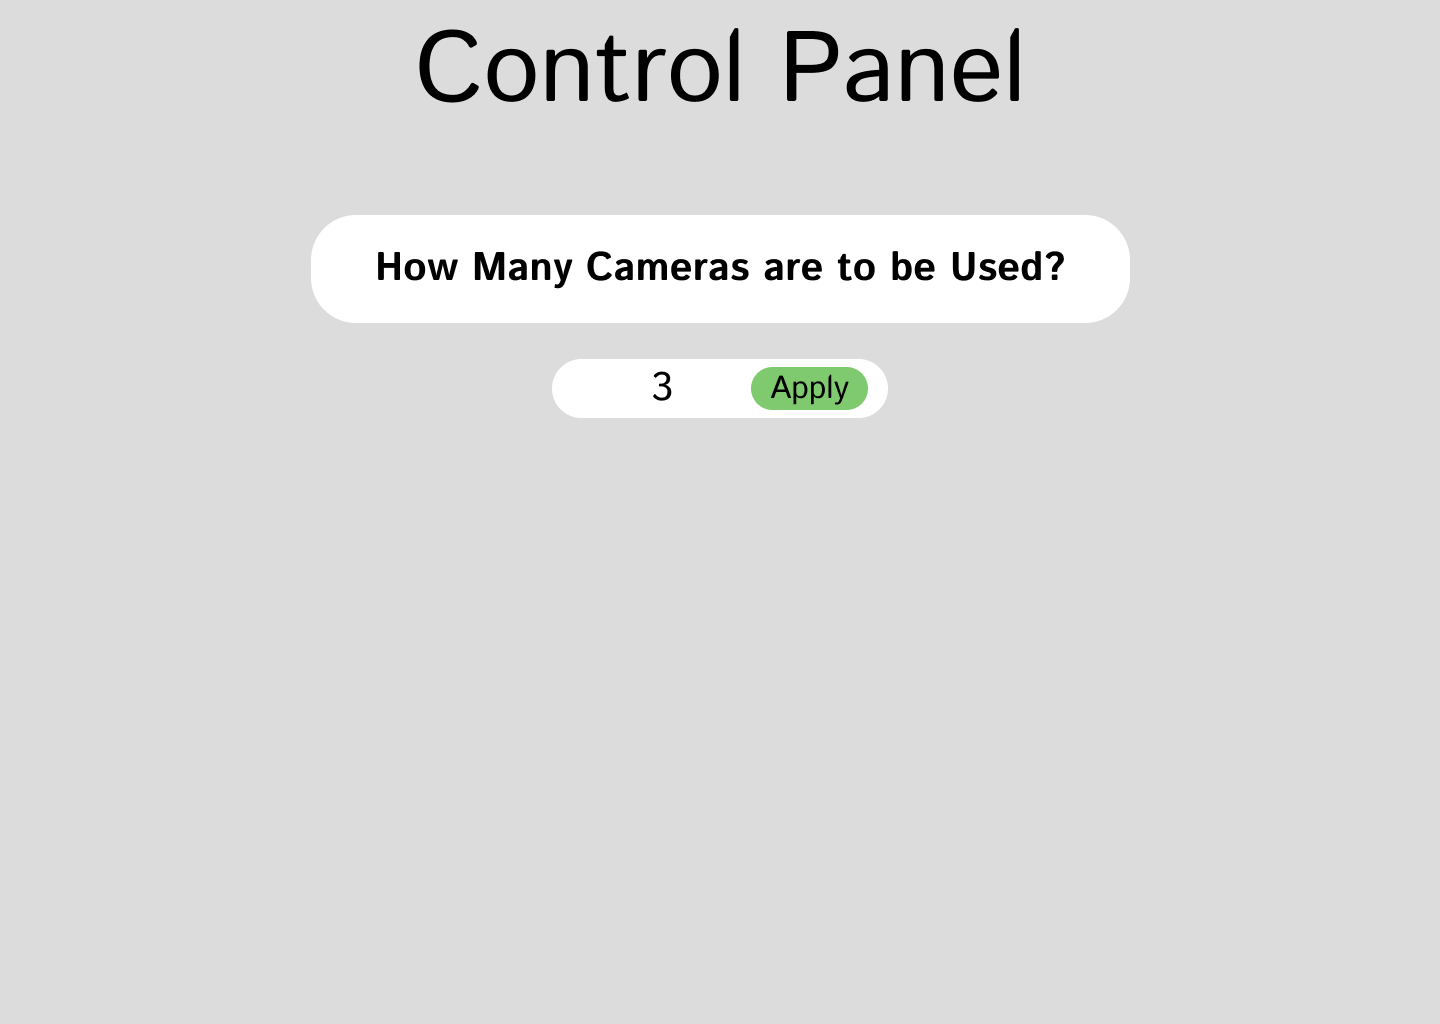
\includegraphics[width=\linewidth]{figures/methods/wireframes/control-panel-1.png}
        \caption{Step 1}
        \label{fig:control-panel-1}
    \end{subfigure}
    \hfill
    \begin{subfigure}[h!]{0.40\linewidth}
        \centering
        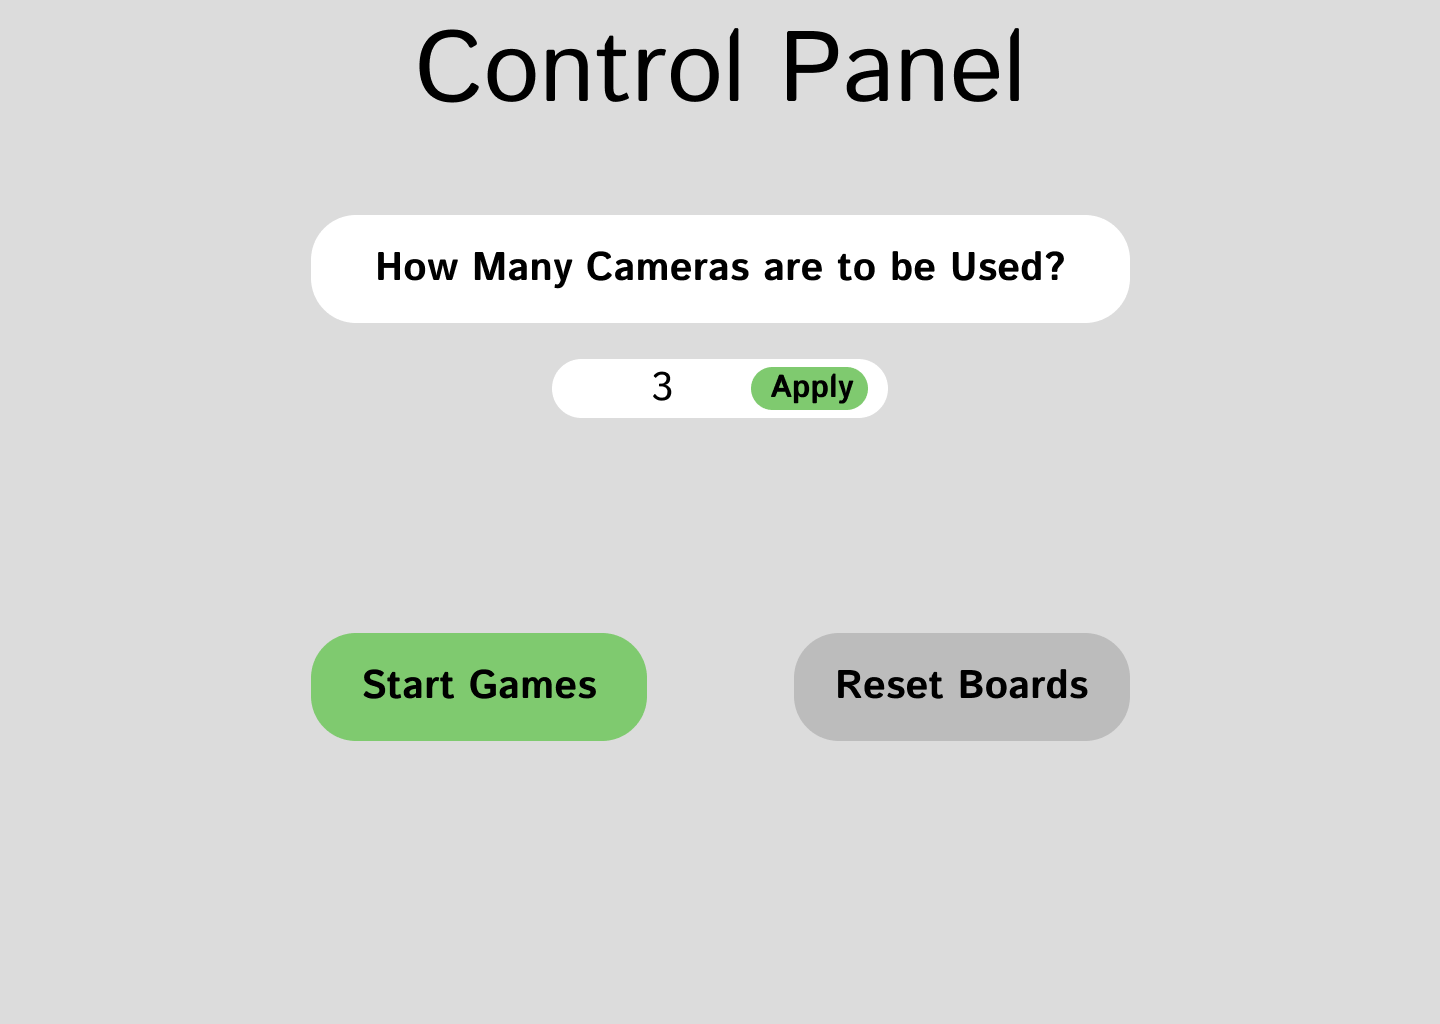
\includegraphics[width=\linewidth]{figures/methods/wireframes/control-panel-2.png}
        \caption{Step 2}
        \label{fig:control-panel-2}
    \end{subfigure}

    \begin{subfigure}[h!]{0.40\linewidth}
        \centering
        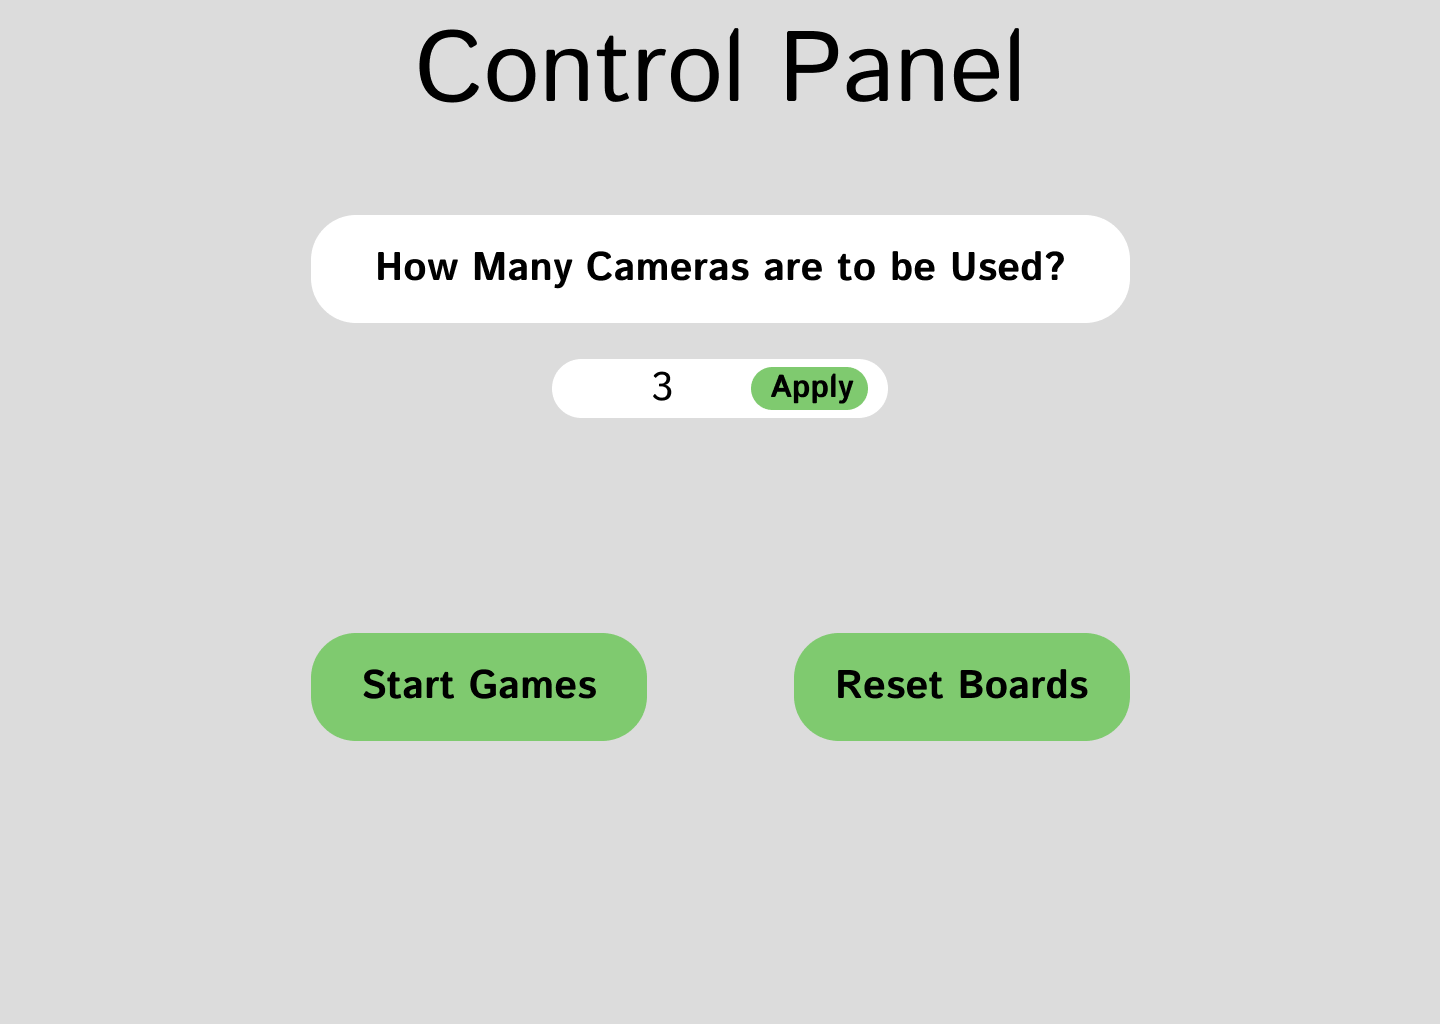
\includegraphics[width=\linewidth]{figures/methods/wireframes/control-panel-3.png}
        \caption{Step 3}
        \label{fig:control-panel-3}
    \end{subfigure}
    
    \caption{Control Panel wireframes showing sequential interaction steps}
    \label{fig:control-panel-group}
\end{figure}


The client-side view is implemented as a web-based interface, developed in accordance with the accessibility principles described in Subsection~\ref{subsec:wcag} of Chapter~\ref{chp:theory}. The design prioritizes usability, aiming to offer a clear, intuitive, and accessible experience for users across both desktop and mobile platforms. \\

The interface is organized into two primary components: the \textbf{Tournament View} and the \textbf{Board View}. \\

The \textbf{Tournament View} (see Figure~\ref{fig:desktop-tournament-view}) provides a concise overview of all active games in the tournament. Its clean and minimal layout presents key information such as board numbers, player names, and a navigation button for accessing the corresponding Board View. This approach ensures that users can quickly scan through the tournament and access matches with minimal effort. \\

The \textbf{Board View} (see Figure~\ref{fig:desktop-board-view}) is focused on a single game, displaying both the live chessboard and a video stream of the ongoing match. The layout is designed for clarity, minimizing distractions so that users can easily follow the game in progress. \\

To ensure compatibility with mobile devices, the interface incorporates responsive design principles. On smaller screens, the \textbf{Tournament View} simplifies its presentation by removing player names and retaining only the board number and navigation button (see Figure~\ref{fig:phone-tournament-view}). This streamlined layout maintains usability without overwhelming the limited screen space.
Similarly, the \textbf{Board View} adjusts to a vertical layout on mobile devices, stacking the chessboard and video stream one above the other (see Figure~\ref{fig:phone-board-view}). This configuration enhances readability and preserves the overall clarity of the interface, even on compact displays.


\begin{figure}[h!]
\subsubsection*{Desktop View}
    \centering
    \begin{subfigure}[h!]{0.40\linewidth}
        \centering
        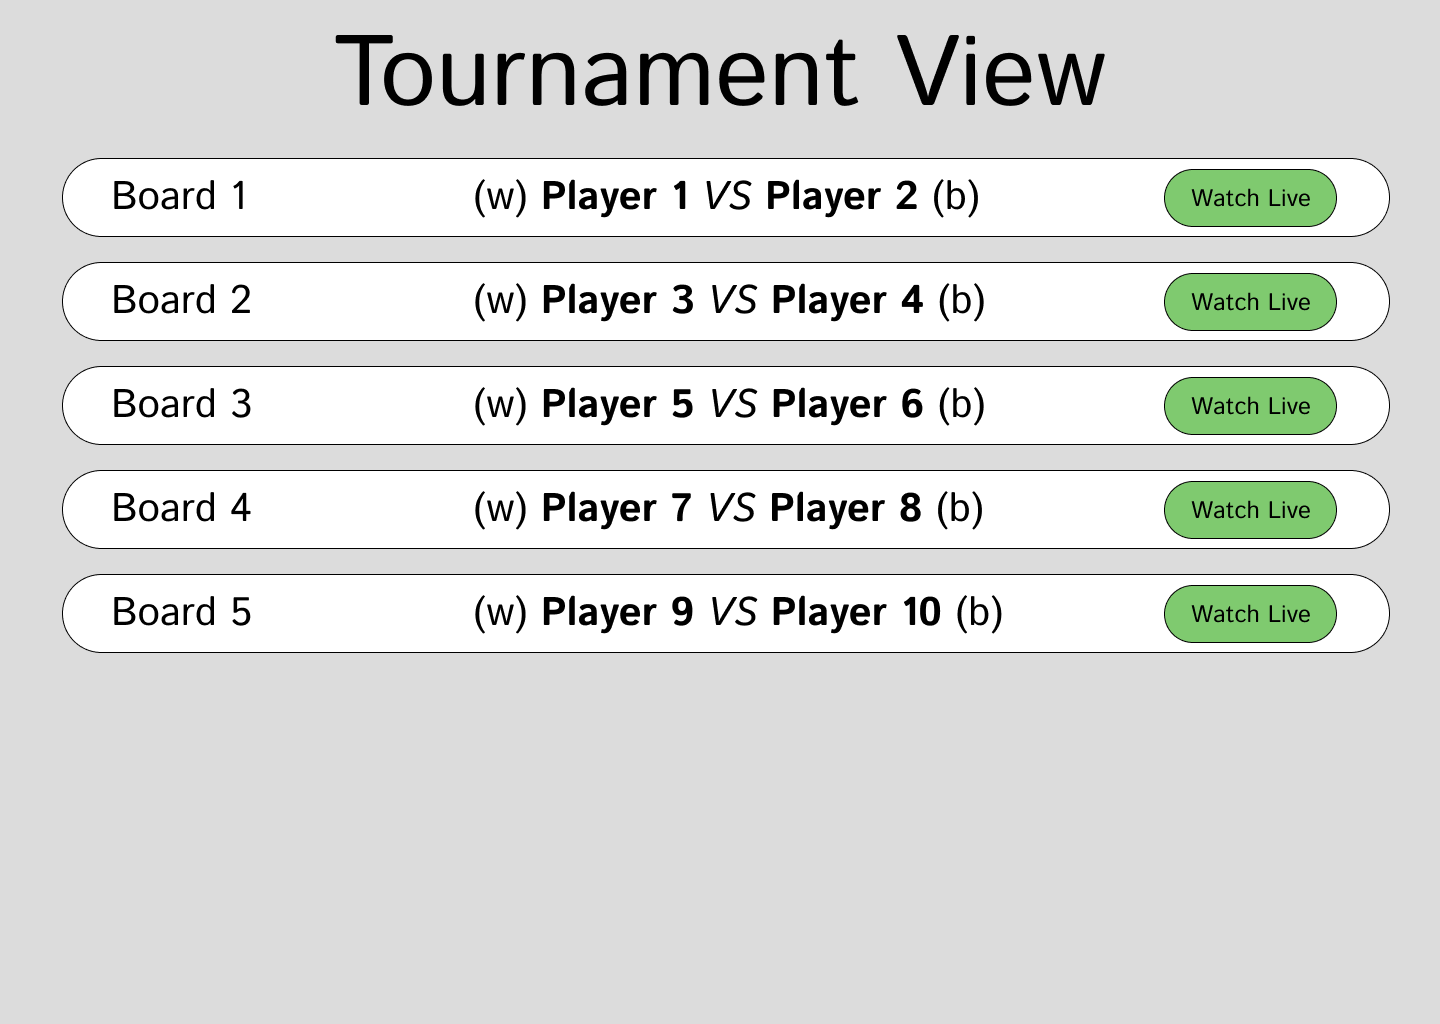
\includegraphics[width=\linewidth]{figures/methods/wireframes/desktop-tournament-view.png}
        \caption{Tournament View}
        \label{fig:desktop-tournament-view}
    \end{subfigure}
    \hfill
    \begin{subfigure}[h!]{0.40\linewidth}
        \centering
        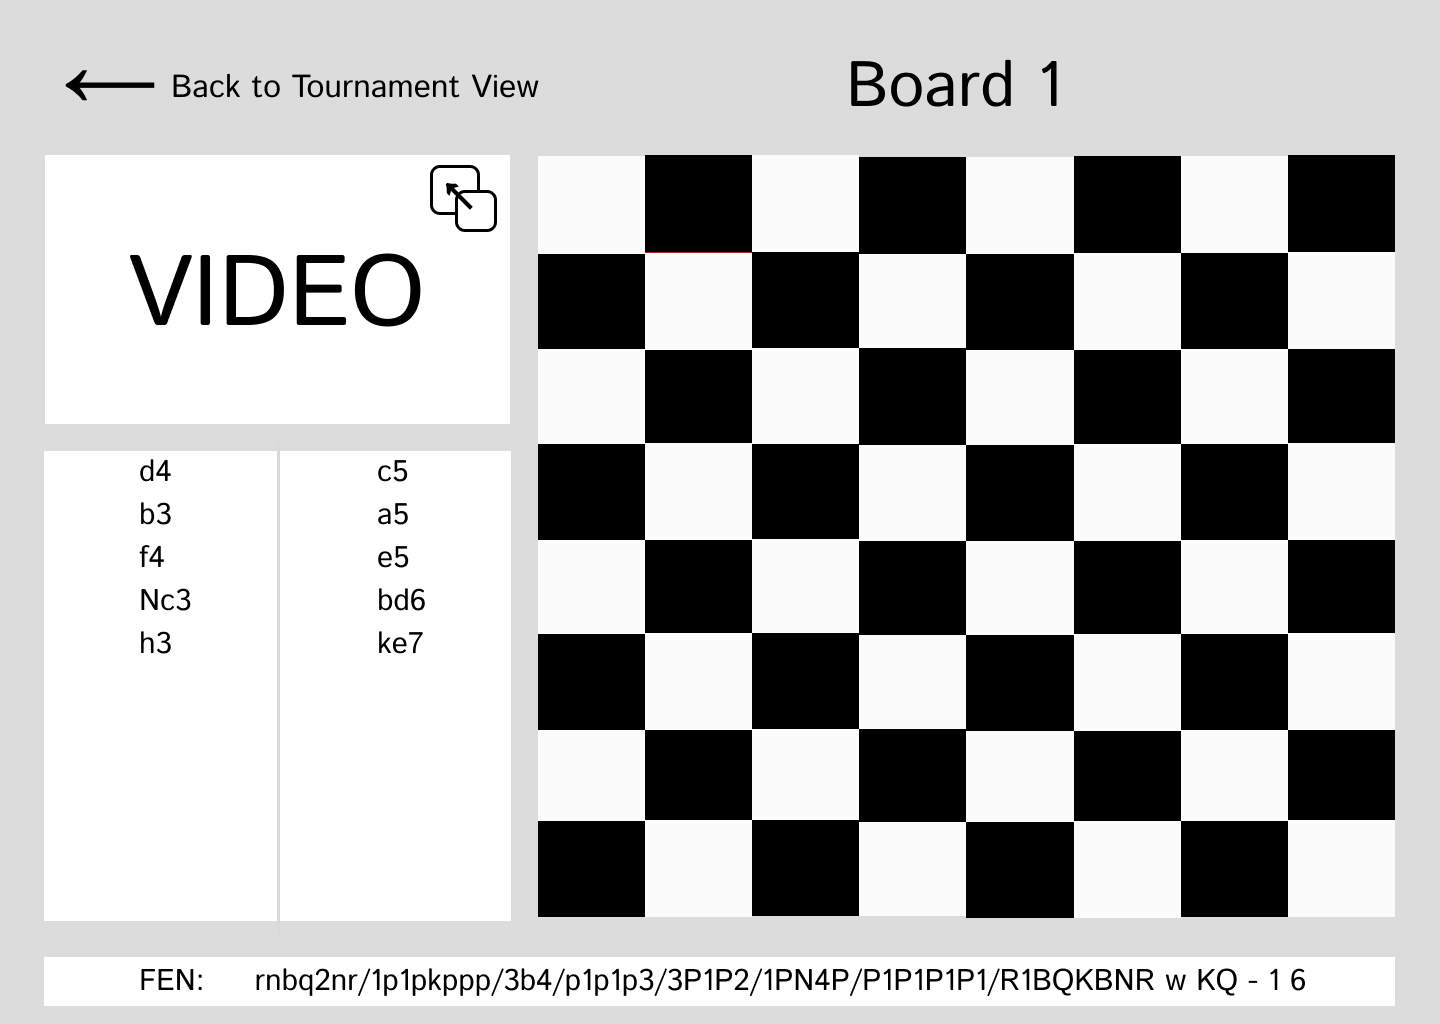
\includegraphics[width=\linewidth]{figures/methods/wireframes/desktop-board-view.png}
        \caption{Board View}
        \label{fig:desktop-board-view}
    \end{subfigure}

    \begin{subfigure}[h!]{0.40\linewidth}
        \centering
        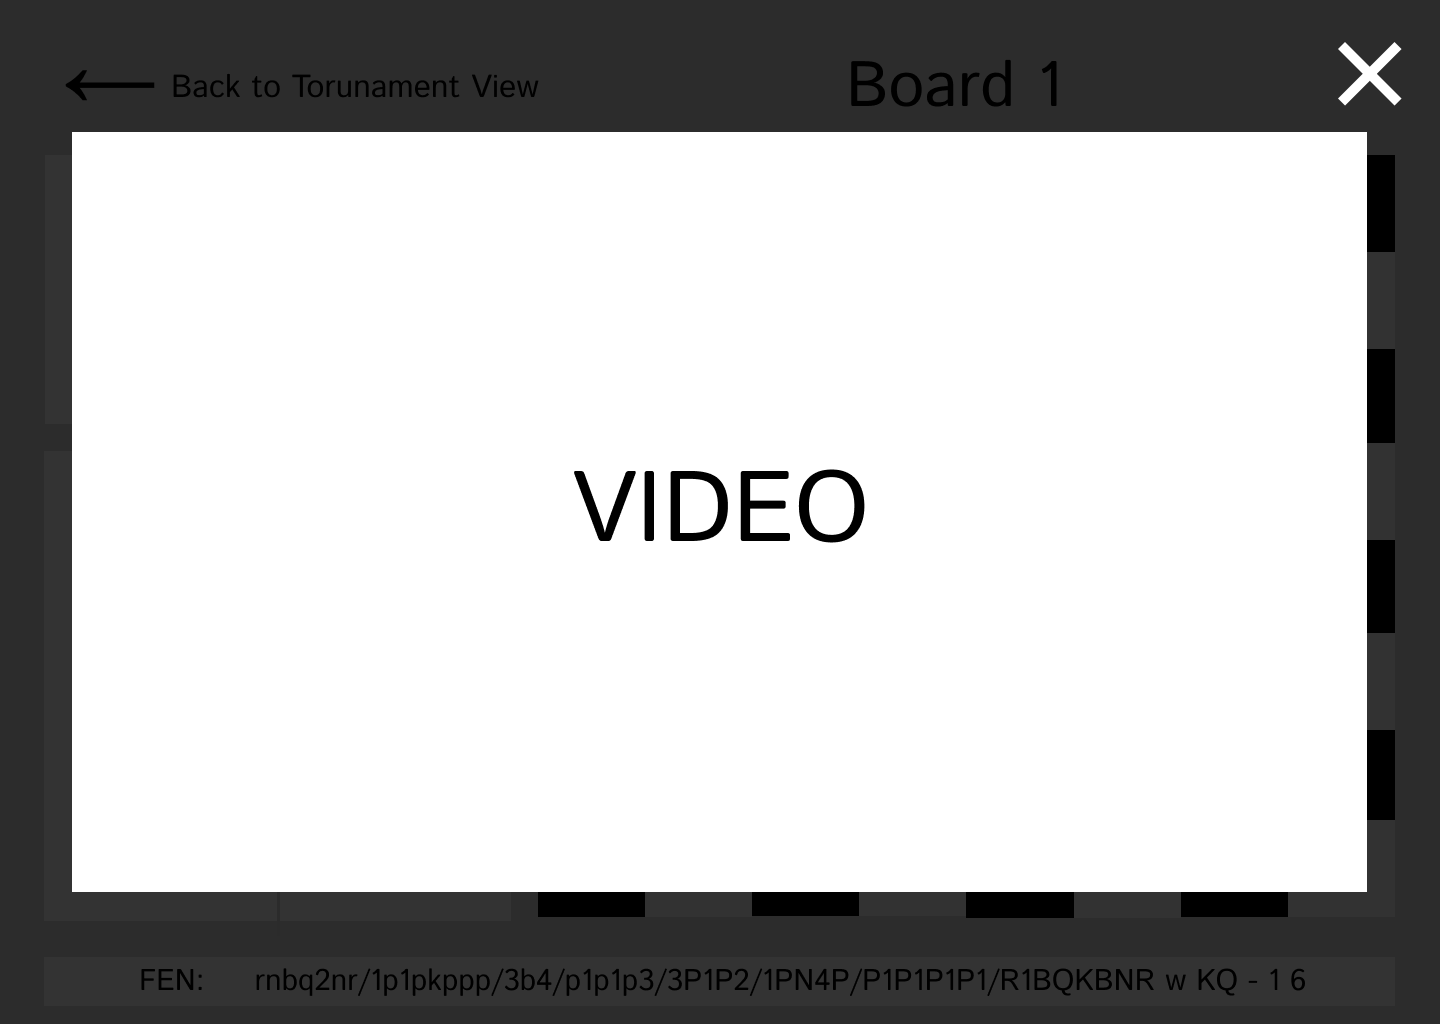
\includegraphics[width=\linewidth]{figures/methods/wireframes/desktop-full-screen-video-view.png}
        \caption{Fullscreen Video Feed}
        \label{fig:desktop-fullscreen-video}
    \end{subfigure}
    
    \caption{Desktop client-side view wireframes}
    \label{fig:desktop-view-group}
\end{figure}


\begin{figure}[h!]
\subsubsection*{Phone View}
    \centering
    \begin{subfigure}[h!]{0.2\linewidth}
        \centering
        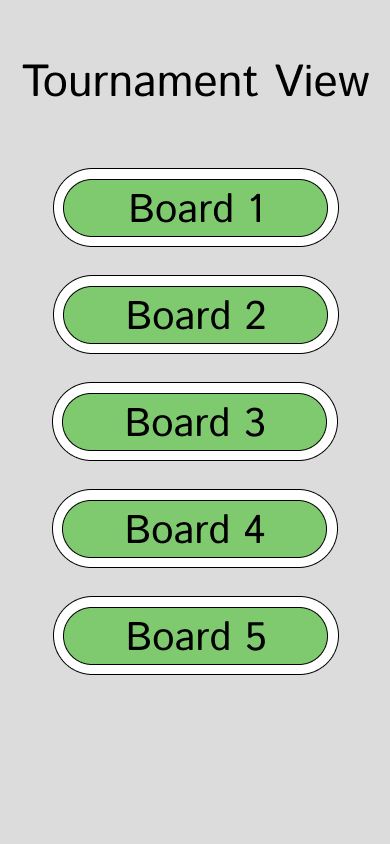
\includegraphics[width=\linewidth]{figures/methods/wireframes/phone-tournament-view.png}
        \caption{Tournament View}
        \label{fig:phone-tournament-view}
    \end{subfigure}
    \hfill
    \begin{subfigure}[h!]{0.2\linewidth}
        \centering
        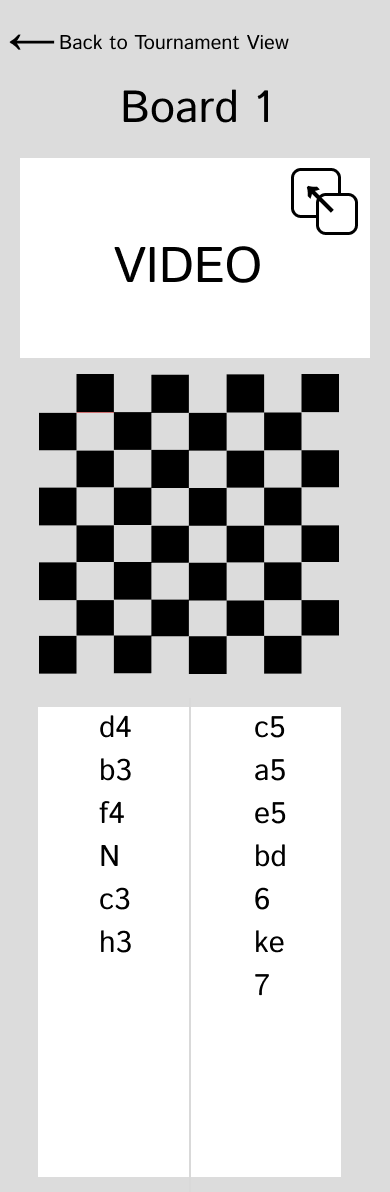
\includegraphics[width=\linewidth]{figures/methods/wireframes/phone-board-view.png}
        \caption{Board View}
        \label{fig:phone-board-view}
    \end{subfigure}
    \hfill
    \begin{subfigure}[h!]{0.2\linewidth}
        \centering
        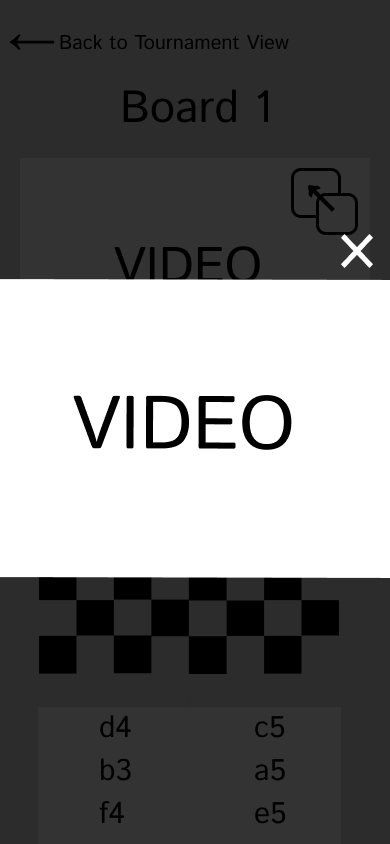
\includegraphics[width=\linewidth]{figures/methods/wireframes/phone-full-screen-video-view-vertical.png}
        \caption{Vertical Fullscreen Video Feed}
        \label{fig:phone-fullscreen-video-vertical}
    \end{subfigure}
    \hfill
    \begin{subfigure}[h!]{0.2\linewidth}
        \centering
        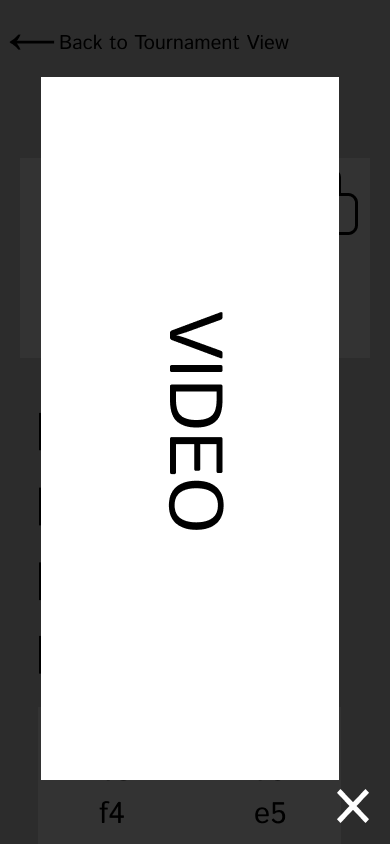
\includegraphics[width=\linewidth]{figures/methods/wireframes/phone-full-screen-video-view-horizontal.png}
        \caption{Horizontal Fullscreen Video Feed}
        \label{fig:phone-fullscreen-video-horizontal}
    \end{subfigure}
    
    \caption{Phone client-side view wireframes}
    \label{fig:phone-view-group}
\end{figure}

\newpage

\section{Project management}
\label{sec:methods-project-management}
The team maintained regular office hours from 10:00 to 16:00 on weekdays, with flexibility for adjustments when necessary. In addition to daily collaboration, the team actively participated in all scheduled meetings with the supervisor and product owner, as well as other relevant events related to the Bachelor project. \\

Most communication took place in person during office hours to support fast feedback and collaboration. When remote communication was needed, particularly outside of regular hours or during individual work sessions, the team used Discord as the primary online platform. \\

The team organized the work into biweekly \textbf{ sprints}, each concluding with a status report and retrospective. At the beginning of each sprint, the product backlog was reviewed to prioritize tasks for the upcoming sprint. Sprint goals were then set, and each team member outlined the tasks they planned to complete before the next meeting. The team reviewed completed tasks to assess progress. For any incomplete tasks, potential causes were discussed, and strategies for addressing them were devised. At the end of each sprint, retrospectives provided an opportunity for the team to reflect on their collaboration and identify areas for improvement. \\

To manage and track tasks, the team utilized GitHub’s \textbf{Issue Board}. Issues were categorized as follows: \textit{Enhancement} for new features or improvements, \textit{Documentation} for adding explanations or improving code safety, \textit{Bug} for errors or unexpected behaviors, and \textit{Task} for general tasks. Each issue was assigned to one or more team members to clarify responsibilities. The Issue Board was organized into four columns: \textit{No Status}, \textit{To Do}, \textit{In Progress}, and \textit{Done}. \\

For \textbf{code review}, the team used GitHub pull requests. Each issue was worked on in a separate branch, enabling team members to review and discuss contributions before merging them into the main codebase.

\section{Tools and Platforms}
\label{sec:tools-and-platforms}

\subsection*{Development Tools}
\label{subsec:development-tools}

\begin{itemize}
    \item \textbf{\acrlong{vscode}} was used as the primary development environment due to its support for multiple programming languages and extensions.
\item \textbf{Postman} was employed for testing and validating \scrshort{rest}ful \glspl{api}, utilizing built-in JavaScript-based test snippets.
\item \textbf{Netron.app} was used to visualize neural network architectures during the evaluation phase.
\item \textbf{Git} facilitated version control and collaboration throughout the development process.
\item \textbf{\glspl{llm}} (e.g., ChatGPT) were consulted to review code and provide suggestions, functioning as a collaborative assistant.
\item \textbf{Lighthouse} was used to evaluate and improve the performance and accessibility of the developed web interface.
\end{itemize}.

\subsection*{Collaboration Tools}
\label{subsec:collaboration-and-design-tools}

\begin{itemize}
    \item \textbf{GitHub} was used for its built-in project management tool, which allowed the team to create an Issue Board for easy issue tracking. It was also used for code reviews and version control management.
    
    \item \textbf{Figma} was used as a tool for sketching and creating wireframes.
    
    \item \textbf{OneDrive} was used as a platform for storing and sharing files.
    
    \item \textbf{Overleaf} was used as the platform for writing the report, utilizing its LaTeX support to efficiently compose and format the thesis.
\end{itemize}


\section{Technology Stack}
\label{sec:technology-stack}

\subsection*{Backend}

Python was selected for the project's backend due to its simple and easy-to-use syntax. Additionally, its extensive ecosystem of libraries and frameworks reduces development time. The language also benefits from its strong community and industry support, providing resources for improving \gls{api} and \gls{ml} knowledge.

\subsubsection*{Python libraries}

\begin{itemize}
    \item \textbf{chess} – Used for move generation, validation, and parsing of chess game formats. \cite{python:chess}
    \item \textbf{FastAPI} – Web framework used to develop \acrshort{rest}ful \glspl{api} for backend services. \cite{python:fastapi}
    \item \textbf{numpy} – Core package for numerical operations. \cite{python:numpy}
    \item \textbf{onnxruntime} Used for running pre-trained machine learning models. \cite{python:onnx}
    \item \textbf{opencv-python} Utilized for computer vision tasks. \cite{python:opencv}
    \item \textbf{requests} – Used to handle \gls{http} communication. \cite{python:requests}
    \item \textbf{scipy} – Employed for scientific and numerical computations. \cite{python:scipy}
    \item \textbf{tensorflow} - Used to build and execute machine learning models. \cite{python:tensorflow}
\end{itemize}


\subsection*{Frontend}

TypeScript was selected for the project's frontend language due to it's type-sefety, as discussed in Subsection \ref{subsec:type-safety} outlined in Chapter \ref{chp:theory}.

\subsubsection*{TypeScript libraries}

\begin{itemize}
    \item \textbf{Vite} is a fast frontend build tool of web applications. \cite{ts:vite}
    
    \item \textbf{React} builds user interfaces out of individual pieces called components. \cite{ts:react}
    
    \item \textbf{\acrshort{swc}} Speeds up the Vite development server. \cite{ts:swc}
    
    \item \textbf{chess.ts} a Typescript chess library for chess move generation/validation, piece placement/movement, and check/checkmate/draw detection \cite{ts:chess}
    
    \item \textbf{react-dom} serves as the entry point to the DOM and server renderers for React. \cite{ts:react-dom}
\end{itemize}

\section{Testing}
\label{sec:testing}

\subsection{Model testing}
\label{subsec:model-testing}

The performance of the machine learning model was evaluated through 100 test games. Five distinct chess openings were selected, with 10 games played per opening on each of two board types: plastic and wooden. This resulted in 50 games per board type. Each game consisted of 15 full moves, corresponding to 15 moves by white and 15 moves by black. \\

Each move was logged as either successful or unsuccessful. A 30-second window was provided for the model to detect and transmit each move, starting from the moment the move was made \gls{otb}. If the model failed to detect the move within this time frame, or if it detected the wrong move, it was marked as unsuccessful. The game concluded either when a move was marked unsuccessful or all 15 full moves had been completed. \\

The webcam was mounted above the board at an angle of approximately 60–70\si{\degree}
 relative to the table surface. The white pieces were placed on the left side of the camera's field of view, and the black pieces on the right.

\begin{figure}[h!]
    \centering
    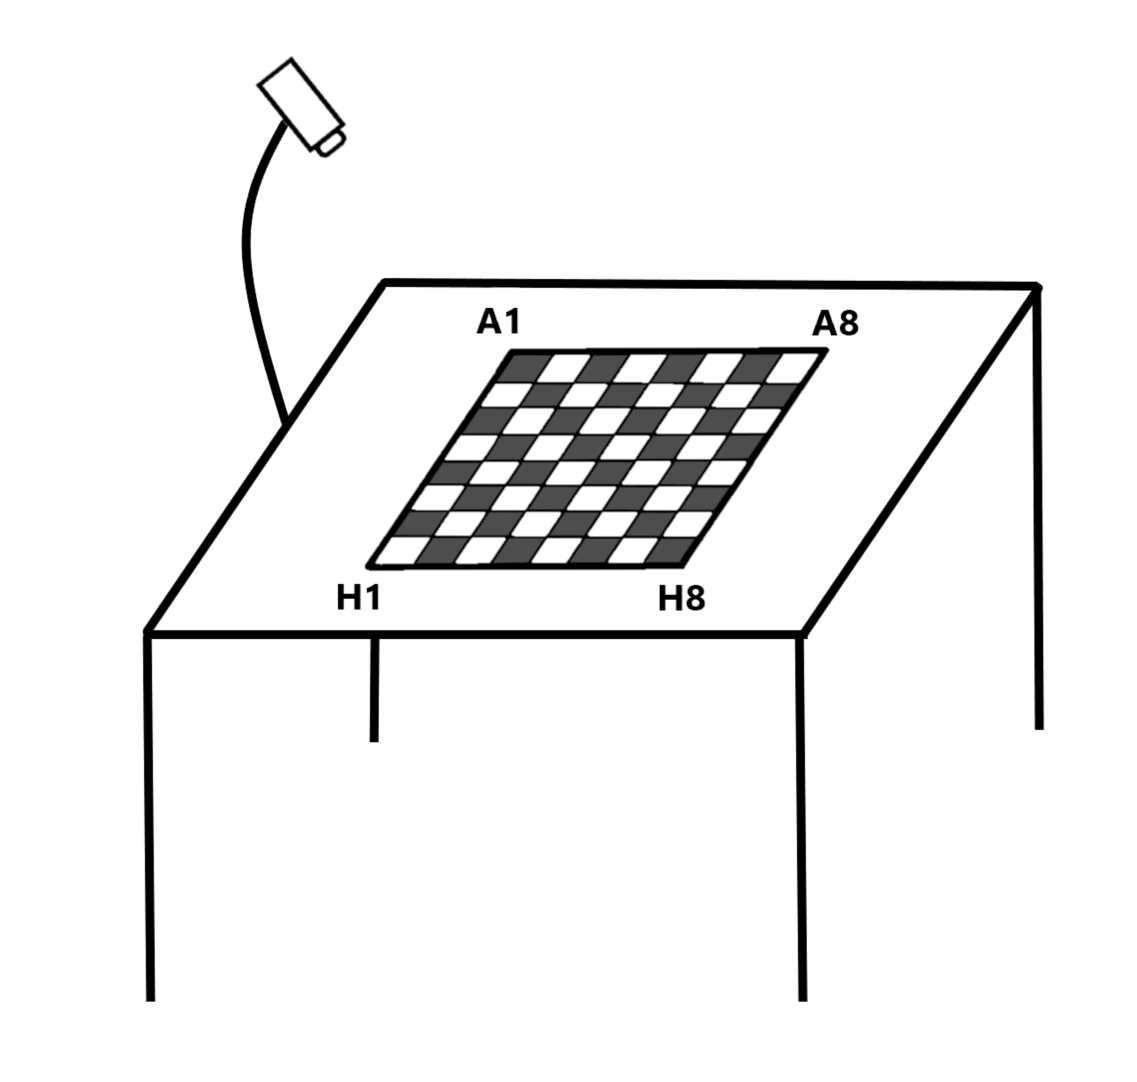
\includegraphics[width=0.75\linewidth]{figures/methods/testing/setup.png}
    \caption[Setup during testing]{Physical setup during testing, showing the board, webcam position, and piece orientation.}
    \label{fig:setup}
\end{figure}



\subsection{Wireframe testing}
\label{subsubsec:user-centered-design}

The following processes align with the principles discussed in  Subsection~\ref{subsec:usability-testing} 
outlined in Chapter~\ref{chp:theory}. At the beginning of the design process, the group conducted wireframe testing with a diverse set of users. This included participants of varying age groups from young to elderly as well as both chess players and non-chess players. The goal was to evaluate whether users found the interface intuitive and whether the sizing and layout were appropriate. \\

All participants were given the same context before starting the test: 

\begin{quote}
\textit{You are viewing a chess game between two companions you know. You visit the tournament organizer's website and come across this webpage.}
\end{quote}

Participants were then either given specific tasks to perform within the application or asked to explore freely, mimicking a real-world scenario. This approach aimed to identify how naturally users could navigate and understand the application without explicit instruction. \\

After completing their interaction with the application, participants filled out an anonymous feedback form. The form included the following questions:

\begin{itemize}
    \item \textit{On a scale from 1 to 5, how satisfied are you with the overall experience of the application?}
    \item \textit{On a scale from 1 to 5, how satisfied are you with the Tournament View page?}
    \item \textit{On a scale from 1 to 5, how satisfied are you with the Board View page?}
    \item \textit{Do you have any feedback, suggestions for improvement, or features you would like to see added?}
\end{itemize}

See Subsection \ref{subsec:wireframe} for the final tested wireframe.

\subsection{Color palette testing}
\label{subsubsec:color-palette}

In selecting the application’s color palette, the group opted for a variation of blue. This choice was influenced by the symbolic associations of the color blue, which is often linked to imagination, intelligence, and wisdom \cite{blue}—traits that are relevant to the game of chess \cite{chess:ppqty, chess:chess-and-creativity}. \\

To identify the most suitable stylistic direction, several versions of the application were developed, each showcasing a distinct color palette. These prototypes were printed and displayed in a shared space, allowing individuals from diverse backgrounds to view and compare them. Participants were invited to vote for their preferred versions via a form. Each participant was allowed up to three votes and had the option to leave comments.



% In selecting the application's color palette, the group opted for a variation of blue. This choice was influenced by the symbolic associations of the color blue, which is often linked to imagination, intelligence, and wisdom \cite{blue} traits that are relevant to the game of chess \cite{chess:ppqty, chess:chess-and-creativity}. \\

% To identify the most suitable stylistic direction, several versions of the application were developed, each showcasing a distinct color palette. These prototypes were printed and displayed in a shared space, allowing individuals from diverse backgrounds to view and compare them. \\

% Participants were invited to vote for their preferred versions via a form. Each participant was allowed up to three votes and had the option to leave comments. For instance, some expressed a preference for the light mode from palette \#08 and the dark mode from palette \#07, while others favored the board design from palette \#05 or the move-highlighting style from palette \#14. \\

% Rather than selecting a single predefined palette, the final color scheme was assembled by combining the most highly rated elements across the top-voted variations. This approach allowed for a more tailored and user-informed visual design (See Figure \ref{fig:color-palette-results} for the vote results). \\

% \begin{figure}[h!]
%     \centering
%     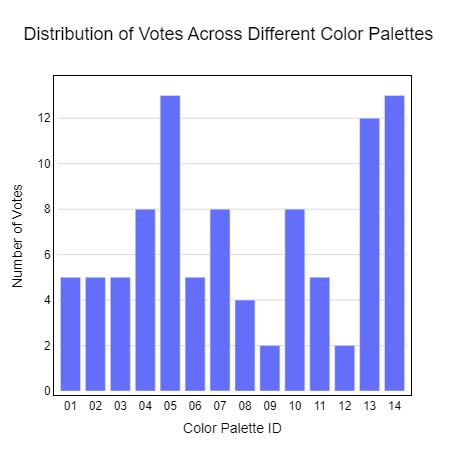
\includegraphics[width=0.75\linewidth]{figures/methods/color-palette-results.png}
%     \caption{Distribution of Votes Across Different Color Palettes}
%     \label{fig:color-palette-results}
% \end{figure}

% See Appendix~\ref{app:color-palettes} for the full set of tested color palettes.